\chapter{Rol and Reference Grammar (RRG)}


The Role and Reference Grammar (RRG) stands as a significant theoretical framework in linguistics, playing a pivotal role in shaping the development of various linguistic theories, including Generalized Phrase Structure (Gazdar et al., 1985), Lexical Functional Grammar (LFG) (Bresnan, 1982, 2001), and Construction Grammar (Fillmore, 1988; Goldberg, 2006). Inspired by typological and theoretical considerations, this approach has left a lasting impact on linguistic scholarship, contributing to the exploration and understanding of diverse linguistic phenomena \parencite{van2009overview}.

\section{Sintactic structure}

The layered structure of a clause (LSC) is grounded in two essential distinctions: firstly, the differentiation between the predicate and non-predicating elements, and secondly, within the realm of non-predicating elements, the distinction between arguments and non-arguments (see Fig. 5.1). This distinction manifests in all languages, irrespective of their configurational nature, whether configurational or non-configurational, head-marking or dependent-marking, free-word-order or fixed-word-order. It encompasses the divide between noun phrases (NPs) and adpositional phrases that function as arguments of the predicate and those that do not \parencite{van1997syntax}. \\


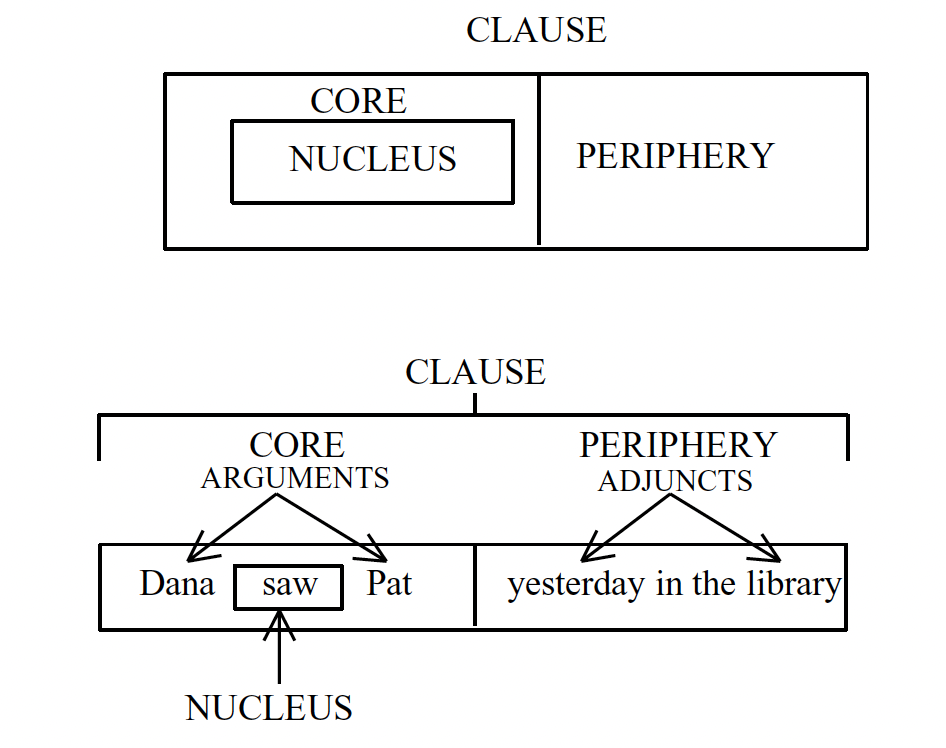
\includegraphics[width=\textwidth]{figures/clausestructure.png}
\captionof{figure}{Extracted from \parencite{van1997syntax} section 1.1, The layered structure of the clause }


In the English sentence, Dana saw Pat yesterday in the library; Dana saw Pat as the core (saw as the nucleus, Dana and Pat as the core arguments). And the library is on the periphery. The clause is divided into a core and a periphery. Within the core, a distinction is made between the nucleus (normally a verb) and its arguments (NPs and PPs, which are
arguments of the predicate in the nucleus). Core arguments are part of the semantic representation of the verb \parencite{van1997syntax}. The
relationships between the semantic and syntactic units are summarized in table 5.1\\

\begin{table}[H]
    \centering
    \begin{tabular}{|p{7cm}|p{4cm}|} \hline 
         \textbf{Semantic element(s)} &  \textbf{Syntactic unit}\\ \hline 
         Predicate & Nucleus\\ \hline 
         Argument in semantic representation of predicate& Core argument\\ \hline 
         Non arguments& Periphery\\ \hline 
         Predicate + arguments& Core\\ \hline 
         Predicate + arguments + Non- arguments& Clause (= core + periphery)\\ \hline
    \end{tabular}
    \caption{Relationships between the semantic and syntactic units}
    \label{tab:my_label}
\end{table}


The RRG (Role and Reference Grammar) conceptualization of the layered structure within a clause represents a semantically-driven perspective on non-relational syntactic structure. This theory posits that the foundational elements in the hierarchical arrangement of sentences and clauses derive their significance from semantic considerations, particularly the contrast between predicate and argument. Furthermore, it extends this semantic motivation to distinguish between XPs (e.g., NPs and PPs) associated with the predicate and those that are not. Thus, the layered structure is intricately shaped by the semantic interplay between predicate-argument relationships and the involvement of XPs concerning the predicate \parencite{van1997syntax}. \\

According to Van Valin (2005), a sentence may include a clause in a detached position, most commonly in the ‘left-detached position’ left [LDP]. This is the location of sentence-initial elements, most commonly adverbials, which are set off from the clause by a pause (See Fig. 5.2), e.g., Yesterday, I bought myself a new car. There is also a ‘right detached position’ [RDP], as in sentences like I know them, those boys. 
When the element in a detached position functions as a semantic verb argument, there is normally a resumptive pronoun in the core referring to it. \\

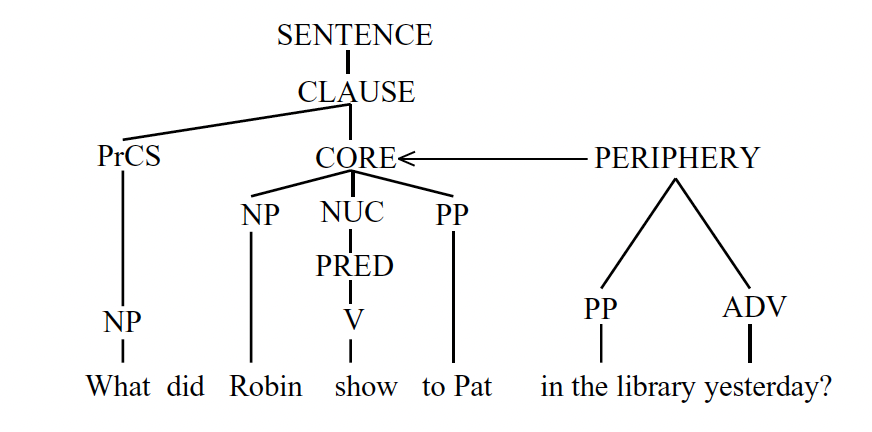
\includegraphics[width=\textwidth]{figures/completeclausestructure.png}
\captionof{figure}{Extracted from \parencite{van1997syntax} section 1.1, The structure of a English clause }

Question words, positioned immediately before the verb, are in the pre-core slot. Within this framework, the presence of an arrow signifies that the periphery functions as an optional modifier of the core.


The distinction between universal and non-universal aspects of clause structure unveils an intriguing observation. The universal elements, encompassing the nucleus, core, periphery, and the clause itself, are all grounded in semantic motivations \parencite{van1997syntax}.\\

In contrast, the non-universal facets, such as detached phrases and extra-core slots, lack semantic motivation; instead, their existence stems from pragmatic considerations \parencite{van1997syntax}. 


\subsection{Operators in the layered structure of a clause}

Grammatical categories such as aspect, tense, and modality are considered operators within the structure, influencing various layers of the clause. Each level of the clause can be subject to modification by one or more operators. The primary operators, or nuclear operators, exert influence over the nucleus, shaping the action, event, or state itself.

In Van Valin (2005), he proposed the following list of operators in LSC. 


\begin{table}[H]
    \centering
    \begin{tabular}{|p{4cm}|p{4cm}|p{4cm}|} \hline
         \textbf{Nuclear Operators} & \textbf{Core Operators} & \textbf{Causal Operators} \\ \hline 
         Aspects&  Directional & Status\\ \hline 
         Negation & Event Quantification & Tense\\ \hline 
         Directionals & Modals & Evidentials\\ \hline 
         &  Internal Negation & Illocutionary Force\\ \hline
    \end{tabular}
    \caption{Operators}
    \label{tab:operators}
\end{table}


Classifying a specific operator as nuclear, core, or clausal is directly determined by its meaning. It's important to note that not all languages necessarily incorporate all of these operators as grammatical categories; their presence depends on each language's linguistic characteristics and features. 
Among the operators, illocutionary force and negation are universal elements in every language. Clausal operators function to modify the entire clause, and they can be categorized into two groups. The first group comprises tense and status; the second includes evidentials and illocutionary force. Notably, negation is the sole operator across all three levels: nuclear, core, and clause.


\subsection{Formal Representation of Clause Structure}

The operators function as modifiers for the core, nucleus, and periphery, distinct from being integral components of these elements. They are represented independently, separate from the predicates and arguments they modify. The ordering of predicates and arguments is subject to language-specific constraints, while the primary guiding principle for arranging operators is the universal scope constraint. \\

Johnson (1987) proposed a formalization of the layered
structure of the clause in which predicates and their arguments are represented in a distinct projection from the one representing operators. This formalization
he termed a ‘projection grammar.’ The schematic depiction of the layered structure of a clause within a projection grammar is illustrated in Fig. 5.3

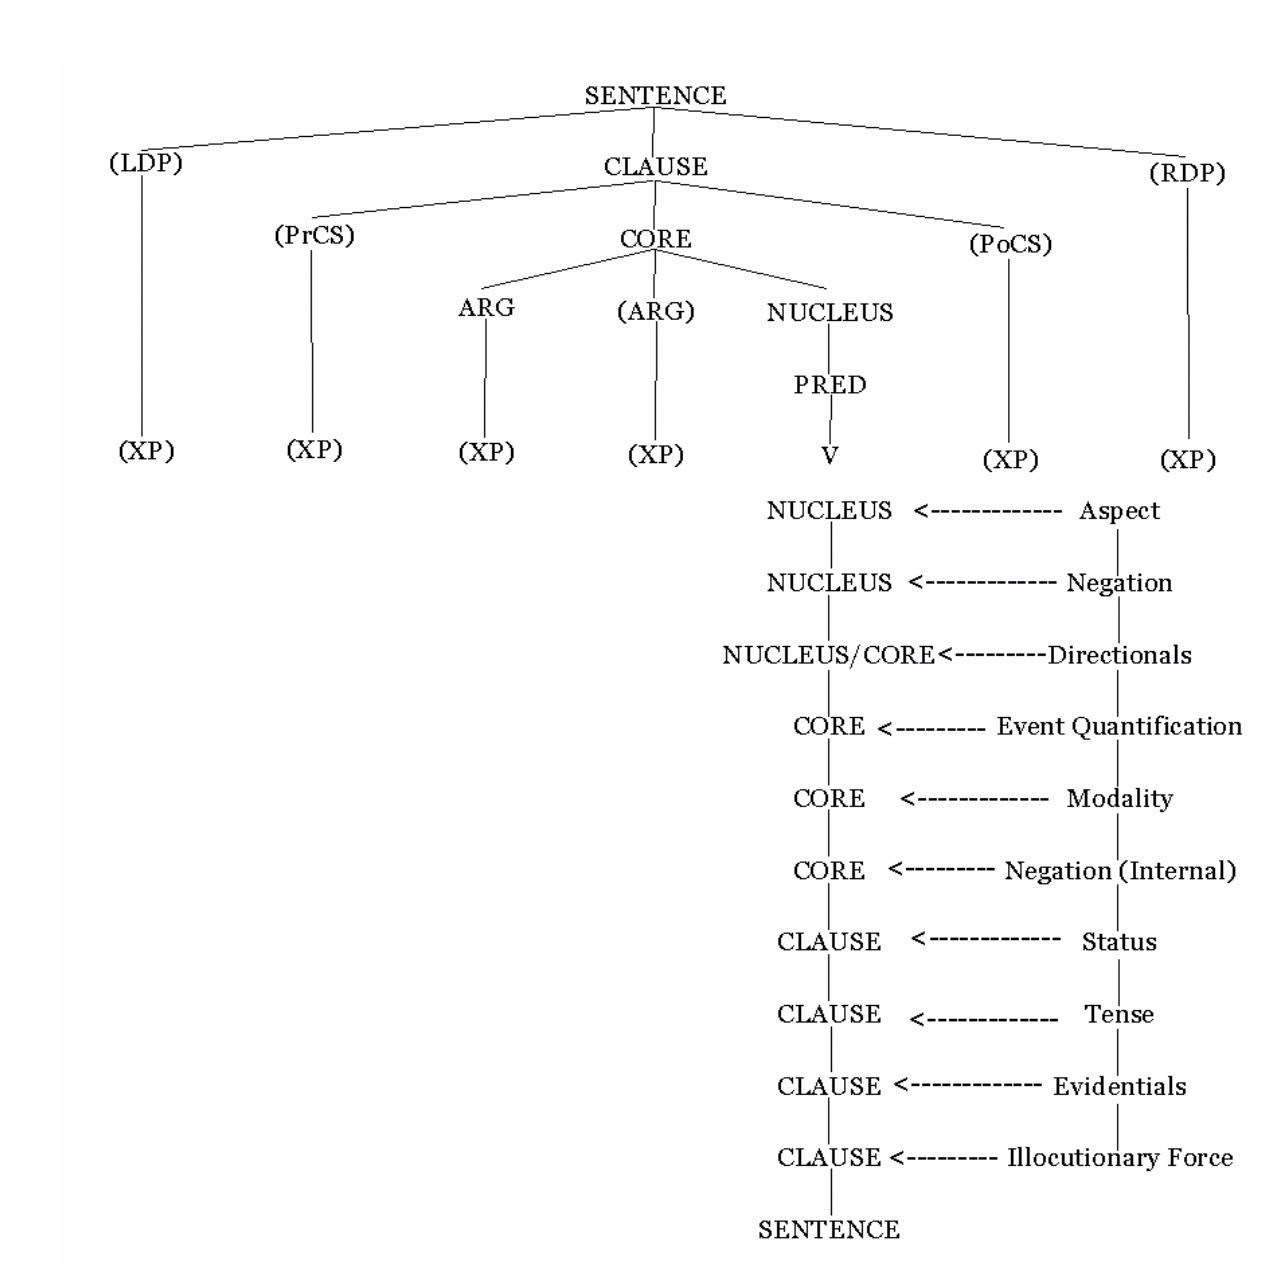
\includegraphics[width=\textwidth]{figures/general-structure-clause.png}
\captionof{figure}{Extracted from \parencite{van1997syntax} section 1.3, Layered structure of the clause with constituent and operator projections}

\subsection{Verb Classes}

In RRG originates from Vendler's (1967) Aktionsart-based categorization of verbs, which classifies them into states, achievements, accomplishments, and activities. RRG incorporates a modified version of Dowty's (1979) representational scheme.

States depict static situations that are inherently temporally unbounded (atelic), and achievements and accomplishments express changes of state, which
are inherently temporally bounded (telic): achievements are instantaneous, while accomplishments are not. Activities are dynamic, inherently temporally unbounded (atelic), states of affairs (\parencite{van1997syntax}).\\

The RRG verbs classification is based on the Aktionsart proposed by Vendler (1967) where verbs are categorized into states, achievements, accomplishments and activities. These four classes can be more precisely delineated by considering three features: [±static], [±punctual], and [±telic] (Binns-Dray, 2004). Static imply if a verb exhibits if something happening. If one answer the question ‘what happened?’ or ‘what is happening?’ then the verb is considered to be static. Telic pertains to whether a verb represents a state of affairs with an inherent terminal point. The last feature, 'punctual,' differentiates events with internal duration from those that lack it. Achievements and accomplishments are telic,or bounded. States and activities are atelic, or unbounded. \\

In addition to the verb classes there are two more,  active accomplishments, which describe telic uses
of activity verbs (e.g. devour), these verbs can be modified by adverbs, and on the other way semelfactives which sometimes describe if the situation involves an action or not (dynamic).\\

Below in table see examples of each class and their formal representation, including their causative counterparts.


\begin{table}[H]
    \centering
    \begin{tabular}{|p{3.5cm}|p{7.5cm}|} \hline 
         \textbf{Verb Classes} & \textbf{Examples}\\ \hline 
         State& be sick, be tall, be dead, love, know, believe, have\\ \hline 
         Activity& march, swim, walk (– goal PP); think, eat (+ mass noun/bare plural
RP)\\ \hline 
         Semelfactive& flash, tap, burst (the intransitive versions), glimpse\\ \hline 
         Achievement& pop, explode, shatter (all intransitive)\\ \hline 
         Acomplishment& melt, freeze, dry (the intransitive versions), learn\\ \hline 
         Active accomplishment& walk (+ goal PP), eat (+ quantified RP), devour\\ \hline
    \end{tabular}
    \caption{Examples of verbs of each class, taken from \textcite{van1997syntax}: 105, based on Example 3.21}
    \label{tab:my_label}
\end{table}



\begin{table}[H]
    \centering
    \begin{tabular}{|p{3.5cm}|p{7.5cm}|} \hline 
         Examples& Causative counterparts\\ \hline 
         State: The boy is afraid.& The dog frightens/scares the boy.\\ \hline 
         Achievement: The balloon popped.& The cat popped the balloon.\\ \hline 
         Semelfactive The pencil tapped on the table.& The teacher tapped the pencil on the table.\\ \hline 
         Accomplishment: The ice melted.& The hot water melted the ice.\\ \hline 
         Activity: The soldiers marched in the park.& The sergeant marched the soldiers in the park.\\ \hline 
         Active accomplishment: The soldiers marched to the park.& The sergeant marched the soldiers to the park.\\ \hline
    \end{tabular}
    \caption{Examples and causative counterparts, taken from \textcite{van2005exploring}: 34 Example 2.5}
    \label{tab:my_label}
\end{table}


\subsection{Lexical representation of verb classes}

An explanation for these patterns can be found in the lexical representations used in RRG: verbs are analyzed in terms of a lexical decomposition system in which state and activity predicates are taken as basic, and the other classes are derived from them.


\begin{table}[H]
    \centering
    \begin{tabular}{|p{3.3cm}  p{7.7cm}|}
     \hline
     \multicolumn{2}{|c|}{} \\ 
         \textbf{Aktionsart class} & \textbf{Logical structure} \\ [.3cm]
         State &  \textbf{predicate'} (x) or (x, y)  \\ [.3cm]
         Activity &  do' (x, [ \textbf{predicate'} (x) or (x, y)] \\  [.3cm]
         Achievement & INGR  \textbf{predicate'} (x) or (x, y), or INGR do' (x[ \textbf{predicate'}(x) or (x, y)])  \\ [.3cm]  
         Semelfative & SEML  \textbf{predicate'} (x) or (x, y) SEML do' (x, [ \textbf{predicate'}(x) or (x, y)]) \\  [.3cm]  
         Accomplishment & BECOME predicate' (x) or (x, y), or BECOME do' (x,[ \textbf{predicate'} (x) or (x, y)]) \\ [.3cm]  
         Active accomplishment & do' (x, [ \textbf{predicate1'} (x, (y))]) \& INGR  \textbf{predicate2'} (z, x) or (y) \\  [.3cm]  
         Causative & $\alpha$ CAUSE $\beta$, where $\alpha$, $\beta$ are logical structures of any type \\  [.3cm]
         \hline
    \end{tabular}
    \caption{Lexical representations for Aktionsart classes, taken from \textcite{van2005exploring} Section 2.1.2 Logical structures,  table 2.3}
    \label{tab:my_label}
\end{table}


These decompositional representations of verbs are referred to as 'logical structures,' the schemas for the classes can be found in Table 5.5. Adhering to the conventions of formal semantics, constants (typically predicates) are presented in boldface, followed by a prime. In contrast, variable elements are presented in normal typeface, often with a (+). The elements in boldface prime form part of the vocabulary of the semantic metalanguage used in the decomposition; they do not correspond to words from any specific human language. Therefore, the same representations are applicable across languages. For instance, the logical structure for Lakhota "t’´a" and English "die" would be "BECOMEdead(x)"  \parencite{van2005exploring}. \\


Examples of some English verbs with their logical structure are presented below in Example 5.2. 


\begin{enumerate}
    \item States
     \begin{enumerate}
        \item Pat is a fool. \\
              \textbf{be'} (Pat, [fool'])
         \item The cup is shattered. \\
         \textbf{shattered'} (cup)
         \item Kim is in the library.\\ 
         \textbf{be-in'} (library, Kim)
         \item Dana saw the picture.\\ 
         \textbf{see'} (Dana, picture)
    \end{enumerate}
    \item Activities
     \begin{enumerate}
         \item The children cried. \\ 
         \textbf{do'} (children, [cry' (children)])
         \item Carl ate pizza. \\
         \textbf{do'} (Carl, [eat'(Carl, pizza)])
     \end{enumerate}
     \item Achievements
     \begin{enumerate}
         \item The window shattered. \\ 
         INGR shattered' (window)
         \item The balloon popped. \\ 
         INGR popped' (balloon)
     \end{enumerate}
     \item Semelfactivities
     \begin{enumerate}
         \item  Dana glimpsed the picture. \\
         SEML see' (Dana, picture)
         \item Mary coughed. \\
         SEML do' (Mary, [cough' (Mary)])
     \end{enumerate}
    \item Accomplishments
     \begin{enumerate}
         \item The snow melted. \\
         BECOME melted' (snow)
        \item Mary learned French. \\ 
        BECOME know' (Mary, French)
     \end{enumerate}
    \item Active accomplishments
    \begin{enumerate}
         \item Chris ran to the park. \\
         do' (Chris, [run' (Chris)]) \& INGR be-at' (park, Chris)
        \item Carl ate the pizza. \\
        do´ (Carl, [eat' (Carl, pizza)]) \& INGR consumed' (pizza)
    \end{enumerate}
    \item Causatives
    \begin{enumerate}
        \item Max melted the ice. \\
        $[do' (dog, \Theta)] CAUSE [feel' (boy, [afraid'])]$  
        \item Max melted the ice. \\
        $[do' (Max, \Theta)] CAUSE [BECOME melted' (ice)]$
        \item The cat popped the balloon. \\
        $[do' (cat, \Theta)] CAUSE [INGR popped' (balloon)]$
        \item Sam flashed the light.  \\
        $[do' (Sam, Ø)] CAUSE [SEML do' (light, [flash' (light)])]$
        \item Felix bounced the ball. \\
        $[do' (Felix, Ø)] CAUSE [do' (ball, [bounce' (ball)])]$
        \item Mary fed the pizza to the child.\\
        $[do' (Mary, Ø)] CAUSE [do' (child, [eat' (child, pizza)])
        \& INGR consumed' (pizza)]$
    \end{enumerate}
\end{enumerate}


\subsection{Semantic roles}

In RRG, two categories of semantic roles, specific and general, are utilized. Specific semantic roles align closely with thematic relations proposed in other theories. The logical structure of a verb serves as a key indicator of its semantic properties, and these properties, as identified by Binns-Dray (2004), determine the corresponding thematic relations.

In addition, according to \textcite{van2005exploring}, the subsequent phase in RRG is refining the semantic representation, which involves defining the semantic relationships between a verb or another predicator and its corresponding arguments.\\

Semantic roles are explored at three distinct levels of generality. The first level encompasses specific roles tied to verbs: runner, killer, hearer, broken, and more. Thematic relations constitute the second level, offering generalizations across these verb-specific roles, including agent, instrument, experiencer, theme, and patient. The third level introduces generalized semantic roles, namely actor and undergoer, which extend across thematic relations \parencite{van2005exploring}. Based on these definitions, in (Example 5.2 1a), Pat is classified as an identified, serving as the first argument of an identificational predication. Meanwhile, the cup is identified as a patient, representing the singular argument in a one-place stative predicate denoting a state or condition. \\

The actor serves in a broad category encompassing roles like agent, experiencer, instrument, and others. In contrast, the undergoer serves as a generalization covering roles such as patient, theme, recipient, and more. The agent is the prototype for the actor, and the patient is the prototype for the undergoes. \\

In the RRG context, two essential semantic roles are proposed: thematic relations and semantic macro roles. These roles are pivotal in the linking system \parencite{van2005exploring}.


\subsubsection{Thematic relations}


\textcite{van2005exploring} states that thematic relations are delineated by referencing the argument positions within the decomposed logical structure representations, a framework influenced by Jackendoff's (1976) work.


\begin{table}[H]
\centering
\begin{tabular}{@{}lll@{}}
\hline
\multicolumn{3}{l}{I. STATES}                         \\
\hspace{2em}A. Single argument    &    &   \\
\hspace{4em}1. State or condition & broken'(x)    & x = patient   \\
\hspace{4em}2. Existence          & exist'(x)     & x = entity    \\
\multicolumn{3}{l}{\hspace{1.5em}B. Two arguments}                  \\
\hspace{4em}1. Pure location & be-LOC'(x, y) & x = location, \\ & & y = theme \\
  \hspace{4em}2. Perception   & hear' (x, y) & x = perceiver, \\ & &
y = stimulus            \\
    \hspace{4em}3. Cognition & know' (x, y) & x = cognizer,  \\ & &
y = content            \\
\hspace{4em}4. Desire & want' (x, y) & x = wanted, \\ & &
y = desire              \\
\hspace{4em}5. Propositional Attitude & consider' (x, y) & x = judged, \\& & y = judgment               \\
\hspace{4em}6. Possession & have' (x, y) & x = possessor, \\ & & y = possessed              \\
\hspace{4em}8. Emotion & love' (x, y) & x = emoter, \\ & & y = target \\
\hspace{4em}9. Attributive & be' (x, [pred']) & x = attributant, \\ & & y = attribute   \\
\hspace{4em}10. Identificational & be' (x, [pred']) & x = identified, \\ & & y = identity \\
\hspace{4em}11. Specificational & be' (x, y) & x = variable, \\ & &
y = value \\
\hspace{4em}12. Equational & equate' (x, y) & x, \\ & & y = referent \\
II. ACTIVITY VERBS  && \\
\hspace{2em}A. Single argument  && \\
\hspace{4em}1. Unspecified action & do' (x, Ø) & x = effector \\
\hspace{4em}2. Motion & do' (x, [walk' (x)]) & x = mover \\
\hspace{4em}3. Static motion & do' (x, [spin' (x)]) &  x = st-mover \\
\hspace{4em}4. Light emission & do' (x, [shine' (x)]) & x = l-emitter \\
\hspace{4em}5. Sound emission & do' (x, [gurgle' (x)]) & x = s-emitter \\
\hspace{2em}B. One or two arguments && \\
\hspace{4em}1. Performance & do' (x, [sing' (x, (y))]) & x = performer, \\ && y = performance \\
\hspace{4em}2. Consumption & do' (x, [eat' (x, (y))]) & x = consumer, \\ &&
y = consumed \\
\hspace{4em}3. Creation & do' (x, [write' (x,(y))]) & x = creator, \\ &&
y = creation \\
\hspace{4em}4. Directed perception & do' (x, [hear' (x, (y))]) & x = observer,  \\ && y = stimulus \\
\hspace{4em}5. Use & do' (x, [use' (x, y)]) & x = user, \\
&& y = implement \\
\hline
\end{tabular}
\caption{Thematic relations}
\label{tab:my-table}
\end{table}


Activity verbs constitute another category of primitive predicates featuring a minimum of ten subclasses. In non-motion activity verbs, the initial argument is an effector—an unmarked participant engaged in an action without specific indications of volition and control. Additional thematic relations linked to the first argument of activity verbs essentially function as subtypes of an effector. Although activity verbs typically prefer a single argument, some exceptions exist with a potential for two arguments, as seen in verbs like eat, drink, and play.


\subsubsection{Macroroles}

The second type of semantic role is the generalized semantic role, the
two macroroles, ‘actor’ and ‘undergoer.’ These constitute the two principal arguments within a transitive predication, and either one has the potential to function as the single argument in an intransitive verb. \\


Examples of actor and undergoer are illustrated below in Example 5.3. \\

\begin{enumerate}
    \item $[\textbf{do'} (Pat, \theta)] \hspace{1em}CAUSE [BECOME \hspace{1em}\textbf{have'} (Chris, book)]$
    \item Pat [actor] gave the book [undergoer] to Chris.
    \item Pat [actor] gave Chris [undergoer] the book.
\end{enumerate}

\textcite{van2005exploring}:61 Example 2.40 \\

The actor represents the argument most akin to an agent, and the undergoer embodies the most reminiscent of a patient. Termed 'macroroles,' these designations encompass various specific thematic relations (See Fig. 5.4). The rationale behind macroroles lies in the observation that grammatical constructions often treat groups of thematic relations similarly.\\

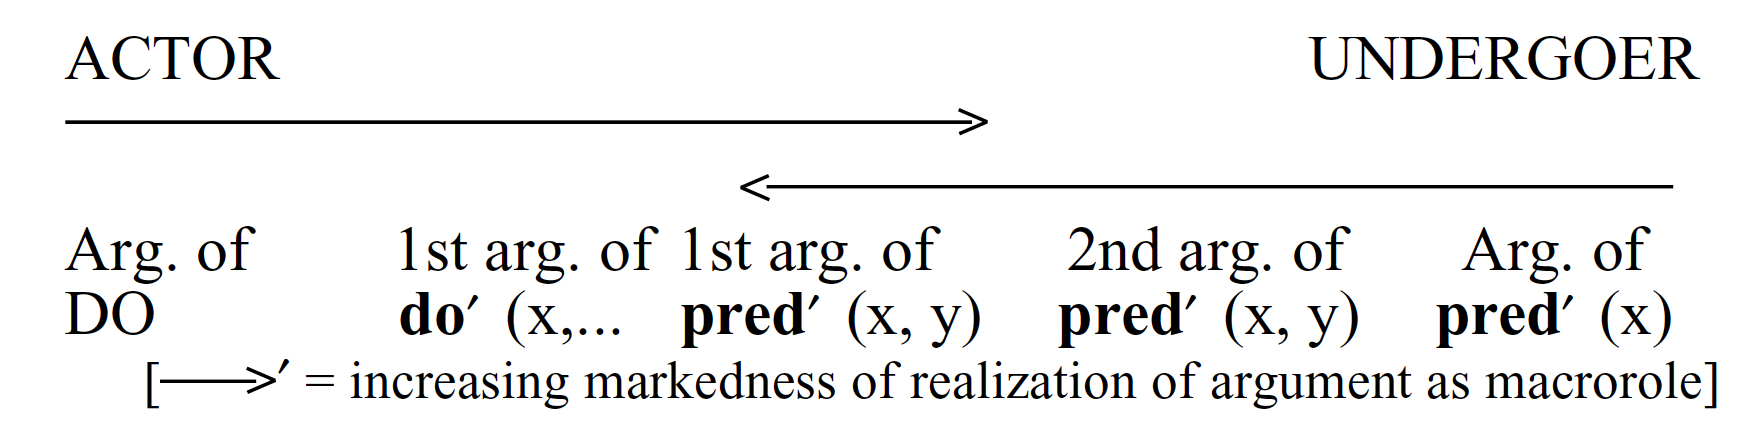
\includegraphics[width=\textwidth]{figures/macroroles-hierarchy.png}
\captionof{figure}{Extracted from \parencite{van2005exploring} section 2.4.2, Actor–undergoer hierarchy (preliminary)} \hfill


The connection between macroroles and logical structure argument positions is encapsulated in the actor-undergoer hierarchy. This principle straightforwardly asserts that, within the logical structure of a transitive verb, the actor is identified as the leftmost argument, while the undergoer is positioned as the rightmost argument.


\section{The Linking System}

The RRG linking algorithm is bidirectional. It establishes a connection between the meaning and structure of language, linking semantic representation to syntactic representation and vice versa.  \\


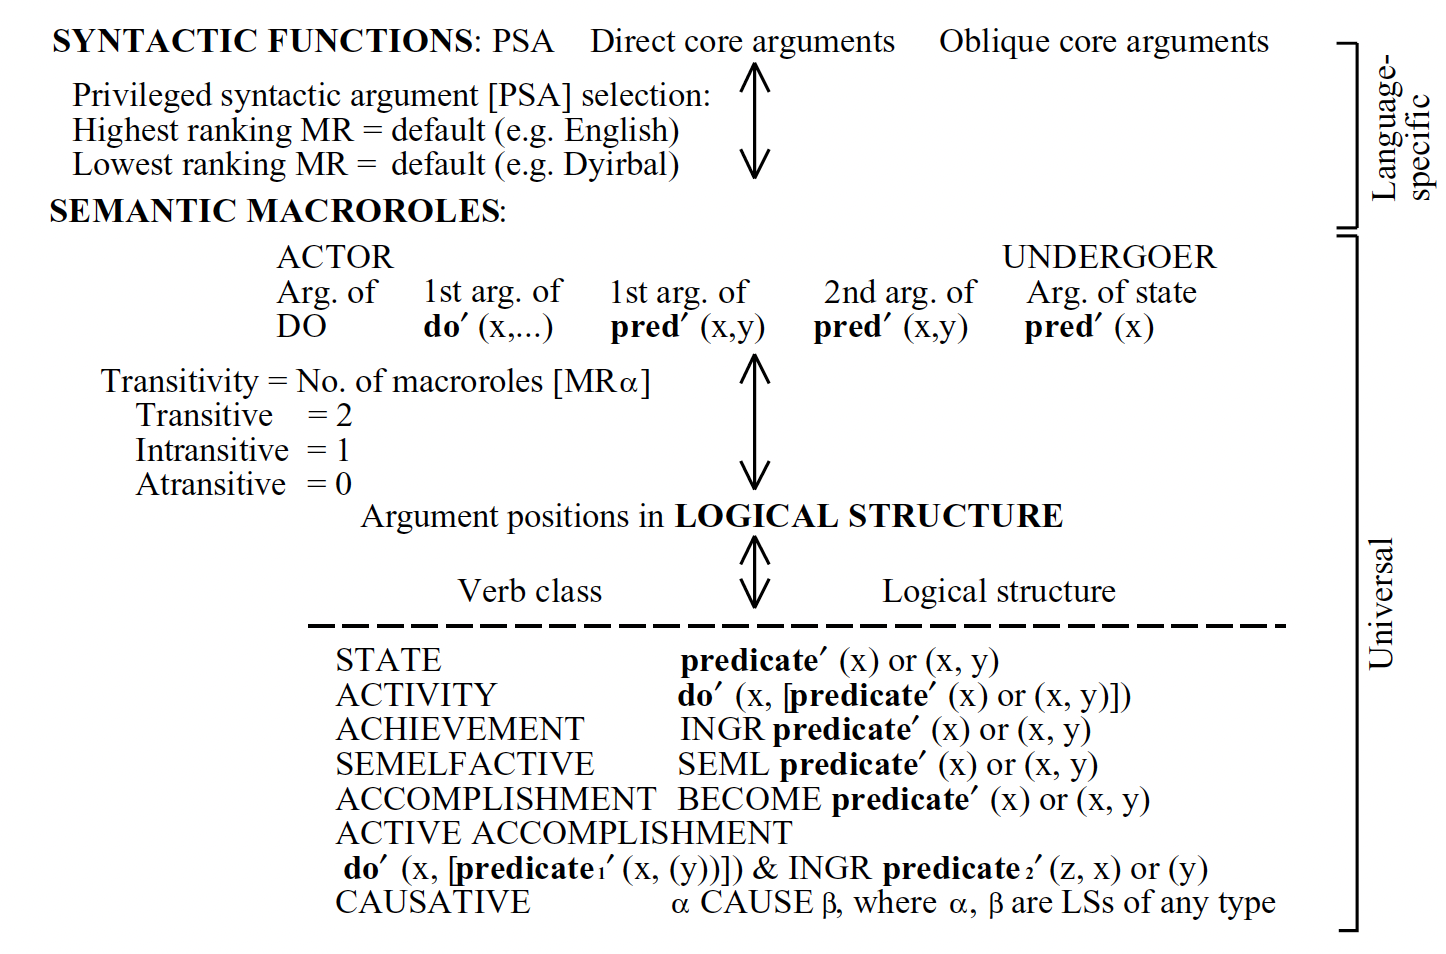
\includegraphics[width=\textwidth]{figures/linking-algorithm.png}
\captionof{figure}{Extracted from \parencite{van2005exploring} section 5.1, Linking algorithm}


Example 5.3 

\begin{enumerate}
    \item Step 1: Construct semantic representation in Lexicon.
    \begin{enumerate}
        \item Access LS for sitting and select prepositional LS to fill be-LOC´ slot in LS, on: \\
        $do' (x sit´ (x, [be-LOC' (y, x)]) + be-on' ( , )]) \\ \implies$
        $do' (x [sit' (x, [be-on' (y, x)])])$
        \item Determine the value of the operators to be expressed:\\
        $<IF DEC <TNS PRES < do' (x, [sit' (x, [be-on' (y, x)])])>>>$
        \item Select the referring expressions to fill the variable positions in LS: \\
        $<IF DEC <TNS PRES < do' (Book, [sit' (Book, ([be-on' (Table, Book))])>>>$
    \end{enumerate}
    \item Step 2: Determine actor and undergoer assignments:\\
    $<IF \hspace{1em} DEC \hspace{1em} <TNS \hspace{1em} PRES < do' (ACT: Book, [sit' (Book, [be-on' (Table, Book)])])>>>$
\item Step 3: Determine the morphosyntactic coding of the arguments:
     \begin{enumerate}
         \item PSA selection: Actor as sole macrorole is selected as PSA.
          \item Actor is assigned nominative case as highest ranking macrorole; 
                preposition on is assigned to the table, which receives dative case due to being the first argument of be-on´, a static location.
          \item As the tense is present, the agreement marking is on the nucleus. The nucleus will agree with the actor since it is the highest ranking macrorole.
     \end{enumerate}
\item Step 4: Select syntactic templates:\\
    \begin{enumerate}
         \item Select the PrCS template, which is obligatory in main declarative clauses.
          \item d. n. a.
           \item Select a two-place core, one place for the nucleus and one for the PP.
            \item Select the non-branching nucleus template.
             \item Select two common noun NP templates and a predicative PP template.
    \end{enumerate}
\item Step 5: Assign LS elements to positions in the syntactic representation:
    \begin{enumerate}
         \item Assign the predicate to the nucleus.
         \item Join the operator projection template to the nucleus and attach the
            morphemes expressing operators to it.
         \item (1.a). Since the nucleus is finite, link it to the first position in the core.
         \item Link the nominative case-actor The Book to the PrCS.
         \item Link the PP to the remaining core position.
\end{enumerate}
\end{enumerate}

\section{Sign\_A framework}

The Sign\_A framework, proposed by \parencite{murtagh2019linguistically}, addresses the absence of a universally accepted standard for documenting Sign Languages (SLs). Developed to facilitate the inclusion of sign languages in the SL lexicon, the framework introduces the 'Articulatory Structure Level' (A). This level, known as the Articulatory Structure Level, expands upon the generative lexicon (GL) theory proposed by Pustejovsky in 1991. \\

Pustejovsky (1995) describes the Generative Lexicon (GL) as a linguistic semantics theory emphasizing the decentralized nature of compositionality in natural language. The GL theory has four main levels of representation. as follows: 


\begin{table}[H]
    \centering
    \begin{tabular}{|p{4cm}|p{7cm}|} \hline 
         Lexical representation level& Description\\ \hline 
         Argument structure& The behavior of a word as a function, with
its arity specified. This is the predicate
argument structure for a word, which
indicates how it maps to syntactic
expressions.\\ \hline 
         Event structure& Identification of the particular event type
(in the sense of Vendler (1967)) for a
word or phrase: e.g., as state, process, or
transition.\\ \hline 
         Qualia structure& The essential attributes of an object as
defined by the lexical item.\\ \hline 
         Inheritance structure& How the word is globally related to other
concepts in the lexicon..\\ \hline
 Articulatory Structure&The essential (computational) phonological
parameters of an object as defined by the lexical
item.\\\hline
    \end{tabular}
    \caption{Five levels of lexical representation for Sign Language Murtagh (2019)}
    \label{tab:my_label}
\end{table}


A fifth level of lexical representation incorporates an object's essential (computational) phonological parameters as defined by the corresponding lexical item. These parameters play a pivotal role in capturing the computational phonological essence of an object. They will be instrumental in addressing diverse linguistic phenomena related to the ISL manual and Non-Manual Features (NMFs). This inclusion is imperative for comprehensively representing ISL within a computational framework \parencite{murtagh-etal-2022-sign}. \\


In contrast, the non-universal facets, such as detached phrases and extra-core slots, lack semantic motivation; instead, their existence stems from pragmatic considerations.

